\documentclass[12pt]{article}
\usepackage[utf8]{inputenc}
\usepackage[T1]{fontenc}
\usepackage{csvsimple}
\usepackage{booktabs}
\usepackage{siunitx}
\usepackage{float}
\usepackage[margin=0.5in]{geometry}
\usepackage{graphicx}
\usepackage{pgfplots}
\usepackage{tikz}
\usepackage{algpseudocode}
\usepackage{amsmath}
\usepackage{algorithm}

\newcommand{\distplot}[4]{
\begin{tikzpicture}
\begin{axis}[
height = 70,
width = 0.8\textwidth,
xbar stacked,
axis y line = none,
axis x line = none,
xmin = 0,
nodes near coords,
every node near coord/.append style={yshift=10pt},
]
\addplot coordinates {(#1,0)};
\addplot coordinates {(#2,0)};
\addplot coordinates {(#3,0)};
\addplot coordinates {(#4,0)};
\end{axis}
\end{tikzpicture}
}

\newcommand{\distplotlegend}[4]{
\begin{tikzpicture}
\begin{axis}[
height = 70,
width = 0.8\textwidth,
xbar stacked,
axis y line = none,
axis x line = none,
xmin = 0,
nodes near coords,
every node near coord/.append style={yshift=10pt},
legend style={at={(0.5,-0.1)},anchor=north,draw=none,column sep=1ex,},
legend columns=-1
]
\addplot coordinates {(#1,0)};
\addplot coordinates {(#2,0)};
\addplot coordinates {(#3,0)};
\addplot coordinates {(#4,0)};
\addlegendentry{Safe};
\addlegendentry{Borderline};
\addlegendentry{Rare};
\addlegendentry{Outlier};
\end{axis}
\end{tikzpicture}
}

\algnewcommand\algorithmicforeach{\textbf{for each}}
\algdef{S}[FOR]{ForEach}[1]{\algorithmicforeach\ #1\ \algorithmicdo}

\pgfplotsset{compat=1.15}
\graphicspath{ {./images/} }
\usetikzlibrary{arrows,decorations.markings}

\title{Types of Examples - nonOrdinal}

\begin{document}

\section{Imbalance}

In real world classification problems, class imbalance is a common occurrence. For example, in medical data, patients suffering from some condition are usually a minority compared to the group not affected by it. Imbalanced data has a negative impact on classifier learning process. Most often, when training on imbalanced data, resulting model is biased in favour for the larger class. Extensive reaserch has been carried out in order to understand the problem and find ways to reduce it \cite{Napierala2016, Blaszczynski2014}. Sampling methods, as well as dedicated learning algorithms were proposed to overcome this problem. Sampling methods can be divided into over-sampling or under-sampling techniques. Over-sampling involves adding artificial examples to minority class. Under-sampling on the other hand is based on removing examples from majority class. Algorithms which are less prone to imbalanced data are usually ensambles -- classifiers consisting of multiple models trained on different data subsets.

The source of imbalance, however, is not always the data itself. Class imbalance may be caused by the procedures used for classifier training. In case of a multiclass classification problem, a typical approach is to reduce it to a number of binary subproblems. This allows to use algorithms designed for binary classification. Unfortunately, such transformation may be the source of imbalance. Figure \ref{img:balanced} shows an example artificial dataset. The data consists of examples described by two numeric features and divided into three classes. There is $150$ examples in each class.

\begin{figure}[H]
\centering
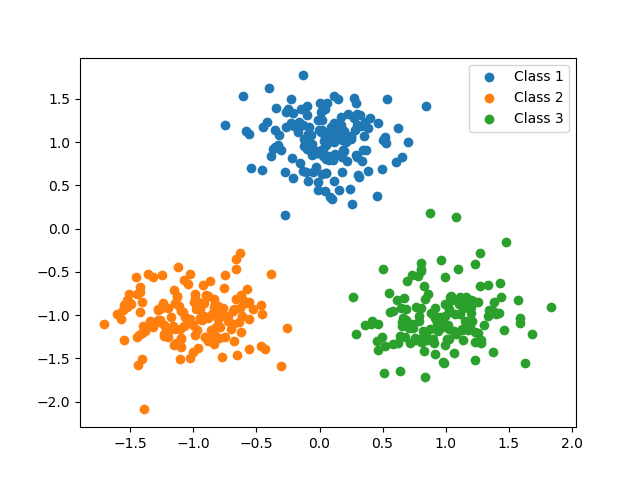
\includegraphics[width=0.6\textwidth]{balanced_data.png}
\caption{Balanced multiclass dataset}
\label{img:balanced}
\end{figure}

In a typical one-vs-rest approach, the problem could be reduced to $3$ binary subproblems. In such case, the training data for every subproblem would be imbalanced with imabalance ratio being $1:2$. Despite the dataset having all of the classes equally numerous, one-vs-rest transformation leads to class imbalance appearing in subproblems training data.

It is also possible for the classes in a multiclass problem to be ordered. In such case, reduction into binary subproblems can be made with regards to the order. A typical approach involves grouping the data into unions. For example, an equally distributed four-class problem would be transformed as shown in Figure \ref{img:balanced_ordered}. Classes in this problem are ordered, with class $Cl_1$ being the least and $Cl_4$ the most preferred.

\begin{figure}[H]
\centering
\begin{tikzpicture}
\draw (0,0) -- (8,0);
\node at (1,-0.6) {$Cl_1$};
\draw (2,0.5) -- (2,-0.5);
\node at (3,-0.6) {$Cl_2$};
\draw (4,0.5) -- (4,-0.5);
\node at (5,-0.6) {$Cl_3$};
\draw (6,0.5) -- (6,-0.5);
\node at (7,-0.6) {$Cl_4$};
\draw [decoration={markings,mark=at position 1 with
    {\arrow[scale=3,>=stealth]{>}}},postaction={decorate}] (4,-1) -- (4,-3);
\end{tikzpicture}

\begin{tikzpicture}
\draw (0,0) -- (8,0);
\node at (1,-0.6) {$Cl_1^\leq$};
\draw (2,0.5) -- (2,-0.5);
\node at (5,-0.6) {$Cl_2^\geq$};
\end{tikzpicture}

\begin{tikzpicture}
\draw (0,0) -- (8,0);
\node at (2,-0.6) {$Cl_2^\leq$};
\draw (4,0.5) -- (4,-0.5);
\node at (6,-0.6) {$Cl_3^\geq$};
\end{tikzpicture}

\begin{tikzpicture}
\draw (0,0) -- (8,0);
\node at (3,-0.6) {$Cl_3^\leq$};
\draw (6,0.5) -- (6,-0.5);
\node at (7,-0.6) {$Cl_4^\geq$};
\end{tikzpicture}
\caption{Ordered multiclass dataset transformation}
\label{img:balanced_ordered}
\end{figure}

Dividing the dataset in this case also causes imbalance. It is worth noting, however, that class imbalance appears when unions border moves closer to the best or the worst class. When the border is placed in the middle, unions are balanced.

In both of the above cases, classes consist of the same number of examples. Such artificial datasets show how imbalance may be caused by the procedures used. In real-world datasets, equal distributions are rarely the case. It is therefore the combination of data characteristics and procedures that influences the imbalance.

\section{Types of minority examples}

In \cite{Napierala2016} a learning example assesment method was introduced. It was designed to estimate learning difficulty for minority class examples in binary classification problem. The method assigns a label to each minority class example. Labels describe the level of learning difficulty and can take one of $4$ values: Safe, Borderline, Rare, Outlier. Assigning labels is therefore a classification task with $4$ classes. The method performs this classification based on each example's neighbourhood.

Originally, the method takes a binary dataset as input. In order to analyze datasets in this study, an extended version of the method was implemented. A simplified outline of this procedure is described in Algorthm \ref{alg:alg1}.

\begin{algorithm}
\caption{Example type classification procedure amended for multiclass dataset}
\begin{algorithmic}
	\State $S \gets build$ $binary$ $subsets$
	\ForEach {$binary$ $subset \in S$}
		\State{$choose$ $minority$ $class$}
		\State{$run$ $example$ $type$ $classification$ $for$ $minority$ $class$}
	\EndFor
\end{algorithmic}
\label{alg:alg1}
\end{algorithm}

An input multiclass dataset is first transformed into a series of binary subsets. For every subset, example type classification is performed on less numerous (minority) class. 

Classification results were saved for every classified example in every subset. After completing the procedure for all subsets, an aggregate statistics could be constructed for entire multiclass dataset.

The key extension of the procedure are transformation methods allowing to obtain binary subsets. Two methods were introduced to be used interchangeably.

\subsection{Union vs. Union Transformation}

The first transformation method is a typical approach visualized in Figure \ref{img:balanced_ordered}. In general case, $n - 1$ binary sets are created for a dataset with $n$ classes. For each class $Cl_t$, where $t \in \{1, n-1\}$ the original dataset is divided into  an upward union $Cl_{t + 1}^\geq$ and downward union $Cl_{t}^\leq$.

\subsection{Class vs. Union Transformation}

The other method divides the original data into subsets consisting of a class and an union. Figure \ref{img:subset} visualizes the divide for an imaginary four-class dataset using this transformation.

\begin{figure}[H]
\centering
\begin{tikzpicture}
\draw (0,0) -- (8,0);
\node at (1,-0.6) {$Cl_1$};
\draw (2,0.5) -- (2,-0.5);
\node at (3,-0.6) {$Cl_2$};
\draw (4,0.5) -- (4,-0.5);
\node at (5,-0.6) {$Cl_3$};
\draw (6,0.5) -- (6,-0.5);
\node at (7,-0.6) {$Cl_4$};
\draw [decoration={markings,mark=at position 1 with
    {\arrow[scale=3,>=stealth]{>}}},postaction={decorate}] (4,-1) -- (4,-3);
\node at (4,-3) {};
\end{tikzpicture}

\begin{tikzpicture}
\draw (0,0) -- (8,0);
\node at (1,-0.6) {$Cl_1$};
\draw (2,0.5) -- (2,-0.5);
\node at (5,-0.6) {$Cl_2^\geq$};
\end{tikzpicture}

\begin{tikzpicture}
\draw (0,0) -- (4,0);
\draw[dotted] (4,0) -- (8,0);
\node at (1,-0.6) {$Cl_1^\leq$};
\draw (2,0.5) -- (2,-0.5);
\node at (3,-0.6) {$Cl_2$};
\draw (4,0.5) -- (4,-0.5);
\end{tikzpicture}

\begin{tikzpicture}
\draw[dotted] (0,0) -- (2,0);
\draw (2,0) -- (8,0);
\draw (2,0.5) -- (2,-0.5);
\node at (3,-0.6) {$Cl_2$};
\draw (4,0.5) -- (4,-0.5);
\node at (6,-0.6) {$Cl_3^\geq$};
\end{tikzpicture}

\begin{tikzpicture}
\draw (0,0) -- (6,0);
\draw[dotted] (6,0) -- (8,0);
\node at (2,-0.6) {$Cl_2^\leq$};
\draw (4,0.5) -- (4,-0.5);
\node at (5,-0.6) {$Cl_3$};
\draw (6,0.5) -- (6,-0.5);
\end{tikzpicture}

\begin{tikzpicture}
\draw[dotted] (0,0) -- (4,0);
\draw (4,0) -- (8,0);
\draw (4,0.5) -- (4,-0.5);
\node at (5,-0.6) {$Cl_3$};
\draw (6,0.5) -- (6,-0.5);
\node at (7,-0.6) {$Cl_4^\geq$};
\end{tikzpicture}

\begin{tikzpicture}
\draw (0,0) -- (8,0);
\node at (3,-0.6) {$Cl_3^\leq$};
\draw (6,0.5) -- (6,-0.5);
\node at (7,-0.6) {$Cl_4$};
\end{tikzpicture}

\caption{Class vs. union transformation}
\label{img:subset}
\end{figure}

In general case, a dataset consisting of $n$ classes is split into $n*2-2$ subsets. In contrary to the previous transformation, subsets do not always contain all of the examples from primary set. Dotted lines in the schema above mark areas not included in a given subset.

\subsection{Neighbourhood Types}

Example type classification is performed on the basis of a classified example's neighbourhood. The number of the same class examples is compared to the number of opposing class examples. The type is determined by the ratio of these two amounts. Two methods for choosing the neighbourhood were used.

\subsubsection{K-Nearest Neighbours}

The first method is based on the kNN algorithm. Given an example from the dataset and a distance metric, the example's neighbourhood is defined as $k$ nearest examples with regards to the metric. $K$ is a parameter of this method, with $5$ being the default value. Since examples in analysed datasets are described by both numeric and nominal attributes, HVDM, introduced in \cite{Wilson1997}, was used as a distance metric.

\subsubsection{Kernel Function}

The second method uses distance thresholding. All examples with the distance to the classified example smaller than a given value, are selected as neighbours. HVDM is also used as a distance metric in this case. The limiting distance value, called \textit{kernel width}, is a method parameter. 

This approach might be less prone to errors in cases of very sparse or dense examples distribution.

\section{Binary Classification Datasets}

Before applying learning difficulty assesment method to multiclass problems, some experiments from \cite{Napierala2016} were replicated in order to verify if own implementation is correct. The same binary classification datasets from UCI repository were used, parameters of the method were also set to be the same as in the original study. Union vs. union transformation was chosen arbitrarly for this experiment, both transformations however do not change the input if it is a binary dataset. As a consequence, the modified procedure should provide similar results to the original one when applied to binary sets.

\subsection{KNN Analysis}

In Tables \ref{tab:knn_own} and \ref{tab:knn_org} own and original results are presented. Table \ref{tab:knn_diff} shows absolute values of differences between corresponding positions. In this experiment, kNN neighbourhood function with $k=5$ was used. Each table is sorted by safe examples percentage in descending order.

\newcolumntype{H}{S[round-mode=places,round-precision=2]}

\begin{table}[H]
\begin{minipage}[t]{0.5\textwidth}
\centering
\csvreader[
    separator=semicolon,
    tabular=lHHHH,
    respect underscore,
    head to column names,
    separator=semicolon,
    table head=\toprule Dataset & S\% & B\% & R\% & O\% \\ \midrule,
    table foot=\bottomrule
]{../results/percentage/nonOrdinal/real/union_vs_union_knn.csv}
{}
{\texttt{\name} & \safe & \borderline & \rare & \outlier}
\caption{Union vs. union - KNN}
\label{tab:knn_own}
\end{minipage}
\begin{minipage}[t]{0.5\textwidth}
\centering
\begin{tabular}{lrrrr}
    \toprule
    Dataset & S\% & B\% & R\% & O\% \\ \midrule
    \texttt{vehicle} & $74.37$ & $24.63$ & & $1.01$ \\
    \texttt{car} & $47.83$ & $39.13$ & $8.70$ & $4.35$ \\
    \texttt{scrotal-pain} & $38.98$ & $45.76$ & $10.17$ & $5.08$ \\
    \texttt{ecoli} & $28.57$ & $54.29$ & $2.86$ & $14.29$ \\
    \texttt{breast-cancer} & $24.71$ & $25.88$ & $32.94$ & $16.47$ \\
    \texttt{transfusion} & $18.54$ & $47.19$ & $11.24$ & $23.03$ \\
    \texttt{cmc} & $17.72$ & $44.44$ & $18.32$ & $19.52$ \\
    \texttt{hepatitis} & $15.63$ & $62.50$ & $6.25$ & $15.63$ \\
    \texttt{abalone} & $8.36$ & $20.60$ & $20.60$ & $50.45$ \\
    \texttt{yeast} & $5.88$ & $47.06$ & $7.84$ & $39.22$ \\
    \texttt{haberman} & $4.94$ & $61.73$ & $18.52$ & $14.81$ \\
    \texttt{solar-flare} & & $48.84$ & $11.63$ & $39.53$ \\
    \texttt{cleveland} & & $31.43$ & $17.14$ & $51.43$ \\
    \bottomrule
\end{tabular}
\caption{Original -- KNN}
\label{tab:knn_org}
\end{minipage}
\begin{minipage}{0.5\textwidth}
\centering
\begin{tabular}{lrrrr}
    \toprule
    Dataset & S\% & B\% & R\% & O\% \\ \midrule
    \texttt{hepatitis} & $21.87$ & $21.87$ & $0$ & $0$ \\
    \texttt{breast-cancer} & $1.18$ & $1.18$ & $1.18$ & $1.18$ \\
    \texttt{abalone} & $0.3$ & $1.5$ & $1.19$ & $0$\\
    \texttt{car} & $0$ & $0$ & $0$ & $0$ \\
    \texttt{cleveland} & $0$ & $5.72$ & $5.72$ & $0$ \\
    \texttt{cmc} & $0$ & $3.3$ & $3.3$ & $0$ \\
    \texttt{ecoli} & $0$ & $2.86$ & $2.85$ & $0$ \\
    \texttt{haberman} & $0$ & $4.94$ & $4.94$ & $0$ \\
    \texttt{scrotal-pain} & $0$ & $1.69$ & $1.69$ & $0$ \\
    \texttt{solar-flare} & $0$ & $2.33$ & $2.32$ & $0$ \\
    \texttt{transfusion} & $0$ & $5.06$ & $5.05$ & $0$ \\
    \texttt{vehicle} & $0$ & $0.51$ & $0.5$ & $0$ \\
    \texttt{yeast} & $0$ & $3.92$ & $3.92$ & $0$ \\
    \bottomrule
\end{tabular}
\caption{Difference -- KNN}
\label{tab:knn_diff}
\end{minipage}
\end{table}

The most significant difference appears for \texttt{hepatitis} dataset. Using own implementation of the classifying method, around $21\%$ more examples were marked as safe. Exactly the same difference appears in borderline percentage, where own method marked less examples. As a conclusion, for this dataset, some of the examples marked as borderline in the original study, were classified as safe in our experiment. 

Almost all of the differences appear to be a transfer between two types of examples. Own implementation tends to mark some of the originally borderline examples as rare. Such differences are visible for \texttt{cleveland}, \texttt{cmc}, \texttt{ecoli}, \texttt{haberman}, \texttt{scrotal-pain}, \texttt{solar-flare},  \texttt{transfusion}, \texttt{vehicle} and \texttt{yeast} datasets.

An equal difference in all $4$ types' percentages was observed for \texttt{breast-cancer} dataset. Here, own method marked less safe and outlier examples in favour of borderline and rare ones.

Overall tendencies, however, appear to be similar. In case of \texttt{car} dataset, results do not differ at all. Apart from \texttt{hepatitis} dataset, in no cases has the difference exceeded $6\%$. 

Differences may have appeared due to data pre-processing. Examples with missing values were deleted from datasets used in this study. It is not known if the data in the original study was also pre-processed and if so, what methods were used. Some implementation differences are also possible and in case of distinction between rare and borderline, additional conditions may have been applied in the original study.

\subsection{Kernel Analysis}

Similar verification experiment was carried out using kernel neighbourhood. Thresholds for classification were set as described in the original study. Kernel width was set per dataset and evaluated as average distance between minority examples and their $5$ nearest neughbours. Results are presented in Table \ref{tab:kernel_own}. Table \ref{tab:kernel_org} shows reference results, differences (absolute values) are shown in Table \ref{tab:kernel_diff}.

\begin{table}[H]
\begin{minipage}[t]{0.5\textwidth}
\centering
\csvreader[
    separator=semicolon,
    tabular=lHHHH,
    respect underscore,
    head to column names,
    separator=semicolon,
    table head=\toprule Dataset & S\% & B\% & R\% & O\% \\ \midrule,
    table foot=\bottomrule
]{../results/percentage/nonOrdinal/real/union_vs_union_kernel.csv}
{}
{\texttt{\name} & \safe & \borderline & \rare & \outlier}
\caption{Union vs. union -- Kernel}
\label{tab:kernel_own}
\end{minipage}
\begin{minipage}[t]{0.5\textwidth}
\centering
\begin{tabular}{lrrrr}
    \toprule
    Dataset & S\% & B\% & R\% & O\% \\ \midrule
    \texttt{vehicle} & $77.4$ & $18.9$ & & $3.7$ \\
    \texttt{car} & $47.8$ & $43.5$ & $8.7$ & \\
    \texttt{ecoli} & $25.8$ & $61.3$ & $3.2$ & $9.7$ \\
    \texttt{scrotal-pain} & $24.4$ & $53.3$ & $11.1$ & $11.1$ \\
    \texttt{breast-cancer} & $18.8$ & $46.3$ & $33.8$ & $1.3$ \\
    \texttt{cmc} & $17.2$ & $44.3$ & $10.4$ & $28.2$ \\
    \texttt{yeast} & $15.2$ & $37.0$ & $2.2$ & $45.7$ \\
    \texttt{haberman} & $15.1$ & $56.2$ & $16.4$ & $12.3$ \\
    \texttt{transfusion} & $15.1$ & $57.8$ & $9.6$ & $17.5$ \\
    \texttt{hepatitis} & $13.6$ & $63.6$ & $9.1$ & $13.6$ \\
    \texttt{abalone} & $7.8$ & $23.7$ & $11.4$ & $57.1$ \\
    \texttt{solar-flare} & $7.1$ & $45.2$ & $7.1$ & $40.5$ \\
    \texttt{cleveland} & $6.7$ & $30.0$ & $13.3$ & $50.0$ \\
    \bottomrule
\end{tabular}
\caption{Original -- Kernel}
\label{tab:kernel_org}
\end{minipage}
\begin{minipage}[t]{0.5\textwidth}
\centering
\begin{tabular}{lrrrr}
    \toprule
    Dataset & S\% & B\% & R\% & O\% \\ \midrule
    \texttt{car} & $26.11$ & $43.5$ & $8.7$ & $26.09$ \\
    \texttt{hepatitis} & $17.65$ & $41.72$ & $15.9$ & $8.28$ \\
    \texttt{vehicle} & $12.07$ & $3.21$ & $3.52$ & $5.35$ \\
    \texttt{scrotal-pain} & $9.15$ & $16.01$ & $2.46$ & $22.8$ \\
    \texttt{transfusion} & $4.99$ & $15.67$ & $15.12$ & $5.53$ \\
    \texttt{breast-cancer} & $4.68$ & $15.71$ & $7.38$ & $12.82$ \\
    \texttt{haberman} & $3.99$ & $36.45$ & $28.04$ & $12.39$ \\
    \texttt{yeast} & $3.44$ & $11.51$ & $11.53$ & $3.32$ \\
    \texttt{abalone} & $3.02$ & $12.66$ & $22.93$ & $7.25$ \\
    \texttt{cmc} & $2.79$ & $11.57$ & $8.22$ & $6.03$ \\
    \texttt{cleveland} & $0.95$ & $12.86$ & $12.41$ & $1.43$ \\
    \texttt{ecoli} & $0.09$ & $15.59$ & $5.37$ & $10.3$ \\
    \texttt{solar-flare} & $0.12$ & $24.27$ & $9.18$ & $15.31$ \\
    \bottomrule
\end{tabular}
\caption{Difference -- Kernel}
\label{tab:kernel_diff}
\end{minipage}
\end{table}

In this case, more significant differences are visible, but overall tendencies still match. The differences could be caused for example by the way Epanechnikov function is utilized to estimate probability or how kernel width is set. The most concerning might be results received for \texttt{car} dataset. In case of kNN variant of the method, results for this dataset were completely aligned with those received in \cite{Napierala2016}. It might indicate that this dataset is identical to the one used in the original study. Since results received using kernel method are different on the same dataset, implementation of this neighbourhood function most probably is the cause of differences.



\subsection{Artificial Datasets}

To further verify the method, the same experiment was carried out on artificially created datasets. The goal was to study the differences of own implementation of kNN and kernel method. K parameter was set to $5$ for kNN neighbourhood, kernel width to average distance to $5$ nearest neighbours of all monority examples in the dataset. The results are presented in Tables \ref{tab:gen_union_knn} and \ref{tab:gen_union_kernel}. Table \ref{tab:gen_union_knn_kernel_diff} shows differences (absolute values). All tables are still sorted by safe percentage in descending order.

\begin{table}[H]
\begin{minipage}{0.5\textwidth}
\fontsize{10pt}{12pt}\selectfont
\centering
\csvreader[
    separator=semicolon,
    tabular=lHHHH,
    respect underscore,
    head to column names,
    separator=semicolon,
    table head=\toprule Dataset & S\% & B\% & R\% & O\% \\ \midrule,
    table foot=\bottomrule
]{../results/percentage/nonOrdinal/gen/union_vs_union_knn.csv}
{}
{\texttt{\name} & \safe & \borderline & \rare & \outlier}
\caption{Union vs. union -- KNN}
\label{tab:gen_union_knn}
\end{minipage}
\begin{minipage}{0.5\textwidth}
\fontsize{10pt}{12pt}\selectfont
\centering
\csvreader[
    separator=semicolon,
    tabular=lHHHH,
    respect underscore,
    head to column names,
    separator=semicolon,
    table head=\toprule Dataset & S\% & B\% & R\% & O\% \\ \midrule,
    table foot=\bottomrule
]{../results/percentage/nonOrdinal/gen/union_vs_union_kernel.csv}
{}
{\texttt{\name} & \safe & \borderline & \rare & \outlier}
\caption{Union vs. union -- Kernel}
\label{tab:gen_union_kernel}
\end{minipage}
\begin{minipage}{0.5\textwidth}
	\fontsize{10pt}{12pt}\selectfont
	\centering
	\csvreader[
	separator=semicolon,
	tabular=lHHHH,
	respect underscore,
	head to column names,
	separator=semicolon,
	table head=\toprule Dataset & S\% & B\% & R\% & O\% \\ \midrule,
	table foot=\bottomrule
	]{../results/percentage/nonOrdinal/gen/knn_kernel_diff.csv}
	{}
	{\texttt{\name} & \safe & \borderline & \rare & \outlier}
	\caption{Union vs. union -- Difference}
	\label{tab:gen_union_knn_kernel_diff}
\end{minipage}
\end{table}

Distributions of the example types received by both kNN and kernel method are similar. The most significant difference was observed for \texttt{flower5-3d-10-20-35-35} dataset, where rare percentage in case of kNN method was about $32\%$ higher. Overall distributions, however, are similar. Kernel method tends to mark more outlier and less rare examples.

The difference in datasets order can be expressed in two position switches. Compared to the results for kNN method, \texttt{paw3-3d-100-0-0-0} in case of kernel neighbourhood is moved one position up, \texttt{flower5-3d-30-40-15-15} is moved two positions up.

It is worth remembering that kernel variant of the method is not expected to return exactly the same results as kNN. While kNN neighbourhood always maintains the same size, kernel function allows the number of neighbours to differ between separate classifications. Size of neighbourhood varies depending on the density of classified example's surrounding. In case of exceptionally dense or sparse neighbourhoods, kNN function may be prone to errors due to arbitrary selection of a fixed number of neighbours. Kernel method takes into account a more significant sample in such cases.

Tables \ref{tab:gen_union_knn_k7} and \ref{tab:gen_union_kernel_2} show a comparison of kNN method with $k=7$ and the same kernel method results (also shown in Table \ref{tab:gen_union_kernel}). Difference is shown in Table \ref{tab:gen_union_k7_kernel_diff}.

\begin{table}[H]
	\begin{minipage}{0.5\textwidth}
		\fontsize{10pt}{12pt}\selectfont
		\centering
		\csvreader[
		separator=semicolon,
		tabular=lHHHH,
		respect underscore,
		head to column names,
		separator=semicolon,
		table head=\toprule Dataset & S\% & B\% & R\% & O\% \\ \midrule,
		table foot=\bottomrule
		]{../results/percentage/k7/nonOrdinal/gen/union_vs_union_knn.csv}
		{}
		{\texttt{\name} & \safe & \borderline & \rare & \outlier}
		\caption{Union vs. union -- KNN, $k=7$}
		\label{tab:gen_union_knn_k7}
	\end{minipage}
	\begin{minipage}{0.5\textwidth}
		\fontsize{10pt}{12pt}\selectfont
		\centering
		\csvreader[
		separator=semicolon,
		tabular=lHHHH,
		respect underscore,
		head to column names,
		separator=semicolon,
		table head=\toprule Dataset & S\% & B\% & R\% & O\% \\ \midrule,
		table foot=\bottomrule
		]{../results/percentage/nonOrdinal/gen/union_vs_union_kernel.csv}
		{}
		{\texttt{\name} & \safe & \borderline & \rare & \outlier}
		\caption{Union vs. union -- Kernel}
		\label{tab:gen_union_kernel_2}
	\end{minipage}
	\begin{minipage}{0.5\textwidth}
		\fontsize{10pt}{12pt}\selectfont
		\centering
		\csvreader[
		separator=semicolon,
		tabular=lHHHH,
		respect underscore,
		head to column names,
		separator=semicolon,
		table head=\toprule Dataset & S\% & B\% & R\% & O\% \\ \midrule,
		table foot=\bottomrule
		]{../results/percentage/k7/nonOrdinal/gen/k7_kernel_diff.csv}
		{}
		{\texttt{\name} & \safe & \borderline & \rare & \outlier}
		\caption{Union vs. union -- Difference}
		\label{tab:gen_union_k7_kernel_diff}
	\end{minipage}
\end{table}

In this case, differences reveal a pattern. The data is sorted by safe percentage, but in Table \ref{tab:gen_union_k7_kernel_diff} outlier differences appear to roughly follow this rule too. Rare percentage differences on the other hand appear in the bottom. Again, kernel method marked more examples as outlier, but less examples as rare.

Link between difference in safe and outlier percentage might indicate that one of the methods is less rigorous or prone to errors. Comparing results for \texttt{flower5-3d-30-70-0-0}, \texttt{paw3-3d-50-50-0-0} and other datasets from upper positions in Table \ref{tab:gen_union_k7_kernel_diff}, it is visible that kNN method with $k=7$ marked more examples as safe and hardly any as outlier. Also, with higher $k$, the differences in general appear to be more significant. Only one value in Table  \ref{tab:gen_union_k7_kernel_diff} is lower than $2\%$. 

In conclusion, the results consistance between kNN method and kernel method is lower for higher $k$ value. The value for $k$ parameter in \cite{Napierala2016} is $5$. In the above experiments too, it appears to perform better than $k=7$.

\section{Ordinal Multiclass Datasets Analysis} \label{ordinal}

The main interest of this study are ordinal multiclass datasets. Number of classes in such datasets can be equal to $2$ or more. Classes can also create an order. For example, an ordinal multiclass dataset can consist of $4$ classes $\{A, B, C, D\}$ which are ordered from the best to the worst. If we assume an order $A > B > C > D$, then $B$ is better than $C, D$ but worse than $A$ ect.

$15$ ordinal multiclass datasets were analysed using the implemented minority example type classification method. The goal of the analysis was to gain overall insight into the data and, more importatly, to verify how introducing order of the classes affects the problem in terms of learning difficulty.

Table \ref{tab:ordinal_properties} presents numbers of examples in each dataset. Total number of examples is shown, along with a per-class distribution. In each case an order of the output classes was defined with no ex-aequo-positioned classes.

\begin{table}[H]
	\fontsize{10pt}{12pt}\selectfont
	\centering
	\csvreader[
		separator=semicolon,
		tabular=lll,
		respect underscore,
		head to column names,
		separator=semicolon,
		table head=\toprule Dataset & Total Examples No.& Per-class Examples No. \\ \midrule,
		table foot=\bottomrule
	]{../results/properties/ordinal/count.csv}
	{}
	{\texttt{\filenames} & \totals & \distributed}
	\caption{Datasets Properties}
	\label{tab:ordinal_properties}
\end{table}

\subsection{Per-dataset Analysis} \label{per_dataset_analysis}

 Combining two variants of neighbourhood functions (kNN, kernel) with two dataset reduction methods (union vs. union, class vs. union) leeds to four experiment setups. Standard parameters were used ($k=5$, kernel width set to mean distance to $5$ nearest neighbours of all minority examples in a dataset). Results for each setup, aggregated into a single distribution per dataset, are presented in Tables \ref{tab:ordinal_union_knn}-\ref{tab:ordinal_class_kernel}. In each table, datasets are ordered by safe percentage.

\begin{table}[H]
\begin{minipage}{0.5\textwidth}
\fontsize{10pt}{12pt}\selectfont
\centering
\csvreader[
    separator=semicolon,
    tabular=lHHHH,
    respect underscore,
    head to column names,
    separator=semicolon,
    table head=\toprule Dataset & S\% & B\% & R\% & O\% \\ \midrule,
    table foot=\bottomrule
]{../results/percentage/ordinal/union_vs_union_knn.csv}
{}
{\texttt{\name} & \safe & \borderline & \rare & \outlier}
\caption{Union vs. union - KNN}
\label{tab:ordinal_union_knn}
\end{minipage}
\begin{minipage}{0.5\textwidth}
\fontsize{10pt}{12pt}\selectfont
\centering
\csvreader[
    separator=semicolon,
    tabular=lHHHH,
    respect underscore,
    head to column names,
    separator=semicolon,
    table head=\toprule Dataset & S\% & B\% & R\% & O\% \\ \midrule,
    table foot=\bottomrule
]{../results/percentage/ordinal/class_vs_union_knn.csv}
{}
{\texttt{\name} & \safe & \borderline & \rare & \outlier}
\caption{Class vs. union -- KNN}
\label{tab:ordinal_class_knn}
\end{minipage}
\begin{minipage}{0.5\textwidth}
\fontsize{10pt}{12pt}\selectfont
\centering
\csvreader[
    separator=semicolon,
    tabular=lHHHH,
    respect underscore,
    head to column names,
    separator=semicolon,
    table head=\toprule Dataset & S\% & B\% & R\% & O\% \\ \midrule,
    table foot=\bottomrule
]{../results/percentage/ordinal/union_vs_union_kernel.csv}
{}
{\texttt{\name} & \safe & \borderline & \rare & \outlier}
\caption{Union vs. union - Kernel}
\label{tab:ordinal_union_kernel}
\end{minipage}
\begin{minipage}{0.5\textwidth}
\fontsize{10pt}{12pt}\selectfont
\centering
\csvreader[
    separator=semicolon,
    tabular=lHHHH,
    respect underscore,
    head to column names,
    separator=semicolon,
    table head=\toprule Dataset & S\% & B\% & R\% & O\% \\ \midrule,
    table foot=\bottomrule
]{../results/percentage/ordinal/class_vs_union_kernel.csv}
{}
{\texttt{\name} & \safe & \borderline & \rare & \outlier}
\caption{Class vs. union -- Kernel}
\label{tab:ordinal_class_kernel}
\end{minipage}
\end{table}

The main observation is that learning difficulty seen as amount of safe examples in a dataset largely varies. Some datasets, like \texttt{car} or \texttt{balance\_scale}, consist of $60\%$ to $80\%$ safe examples (the exact number depends on the method). Other datasets (\texttt{breast-cancer\_nm}) contain significantly less safe examples, especially looking at kernel method results. \texttt{ERA\_n} dataset is described by kernel method as $100\%$ outlier examples.

Per-dataset distributions do not differ much between experiment setups, especially comparing the same neighbourhood functions, but different transformation methods. For datasets like \texttt{breast-w}, \texttt{breast-w\_nm}, \texttt{dataset\_1-noid} or \texttt{breast-cancer\_nm} they are the same for both kNN experiments (Tables \ref{tab:ordinal_union_knn}, \ref{tab:ordinal_class_knn}) and both kernel experiments (Tables \ref{tab:ordinal_union_kernel}, \ref{tab:ordinal_class_kernel}). This can easily be explained by the fact, that these datasets consist of only $2$ classes. In such cases, data transformation is not necessary and classifying method is applied on the datasets in the original form.

\subsection{Per-division Analysis}

Further insight can be gained by analyzing results aggregated per division. Tables \ref{tab:3_union_kernel} and \ref{tab:3_class_kernel} show numbers of examples labelled as given minority type in every division made on texttt{dataset 3}. Classes in this dataset belong to $\{1, 2,3, 4, 5\}$.

\begin{table}[H]
\fontsize{10pt}{12pt}\selectfont
\centering
\begin{tabular}[t]{lllr}
\toprule
Union (min) & Union (maj) &  & Total \\ 
\midrule
$\leq 1$ & $\geq 2$ & \distplot{107}{69}{15}{52} & 243 \\ 
$\leq 2$ & $\geq 3$ & \distplot{241}{108}{4}{186} & 539 \\ 
$\geq 4$ & $\leq 3$ & \distplot{246}{54}{3}{129} & 432 \\ 
$\geq 5$ & $\leq 4$ & \distplotlegend{25}{43}{20}{36} & 124 \\
\bottomrule
\end{tabular}
\caption{\texttt{dataset3} -- Union vs. union, kernel}
\label{tab:3_union_kernel}
\end{table}

\begin{table}[H]
\fontsize{10pt}{12pt}\selectfont
\centering
\begin{tabular}[t]{lllr}
\toprule
Minority & Majority &  & Total \\ 
\midrule
$1$ & $2$ & \distplot{214}{138}{30}{104} & 486 \\ 
$2$ & $3$ & \distplot{152}{68}{4}{72} & 296 \\ 
$3$ & $2$ & \distplot{221}{34}{3}{99} & 357 \\ 
$3$ & $4$ & \distplot{192}{62}{4}{99} & 357 \\ 
$4$ & $3$ & \distplot{189}{35}{4}{80} & 308 \\ 
$5$ & $4$ & \distplotlegend{50}{86}{40}{72} & 248 \\ 
\bottomrule
\end{tabular}
\caption{\texttt{dataset3} -- Class vs. union, kernel}
\label{tab:3_class_kernel}
\end{table}

In Table \ref{tab:3_union_kernel} union vs. union-based subproblems distributions are shown. Since this dataset is not strongly imbalanced, it is visible that in each subproblem the union closer to classes ranking edge happens to be the minority. In Table \ref{tab:3_class_kernel} respective results are shown for class vs. union division method. As noticed in Subsection \ref{per_dataset_analysis}, changing division method does not affect examples difficulty distribution much. Distributions in Table \ref{tab:3_class_kernel} align with those in Table \ref{tab:3_union_kernel} and therefore confirm this observation. Tables \ref{tab:swd_union_kernel} and \ref{tab:swd_class_kernel} below follow this pattern as well.

\begin{table}[H]
\fontsize{10pt}{12pt}\selectfont
\centering
\begin{tabular}[t]{lllr}
\toprule
Union (min) & Union (maj) &  & Total \\ 
\midrule
$\leq 2$ & $\geq 3$ & \distplot{5}{8}{10}{9} & 32 \\ 
$\leq 3$ & $\geq 4$ & \distplot{171}{133}{52}{28} & 384 \\ 
$\geq 5$ & $\leq 4$ & \distplotlegend{56}{106}{38}{17} & 217 \\ 
\bottomrule
\end{tabular}
\caption{\texttt{SWD} -- Union vs. union, kernel}
\label{tab:swd_union_kernel}
\end{table}

\begin{table}[H]
\fontsize{10pt}{12pt}\selectfont
\centering
\begin{tabular}[t]{lllr}
\toprule
Minority & Majority &  & Total \\ 
\midrule
$2$ & $3$ & \distplot{10}{16}{20}{18} & 64 \\ 
$3$ & $4$ & \distplot{326}{252}{102}{56} & 736 \\ 
$5$ & $4$ & \distplotlegend{112}{212}{76}{34} & 434 \\ 
\bottomrule
\end{tabular}
\caption{\texttt{SWD} -- Class vs. union, kernel}
\label{tab:swd_class_kernel}
\end{table}

In this case, it is clearly visible that the amount of safe examples drops the closer the dataset split is to one of classes ranking edges. For subproblems made of an edge class ('2' or '5') and the rest of the dataset, safe examples constitute for around $15\%$ to $25\%$. This is visible in the first and last row of both Table \ref{tab:swd_union_kernel} and \ref{tab:swd_class_kernel}. In case of a subproblem which was made by dividing the dataset closer to the middle of classes ranking, safe examples amount is higher and achieves $44\%$. This confirms the initial intuition, that binary subproblems made by dividing the dataset close to classes ranking edge may pose higher difficulty in learning process. In fact, in case of \texttt{SWD} dataset, this is especially visible since edge classes are the least numerous ones. Therefore, the explanation for high learning difficulty in case of these subproblems may be high imbalance ratio.

It is also possible, however, that the cheracteristic is inverted -- more safe subproblems appear to be the ones with border closer to the edge. Tables \ref{tab:car_union_kernel} and \ref{tab:car_class_kernel} show results for \texttt{car} dataset.

\begin{table}[H]
	\fontsize{10pt}{12pt}\selectfont
	\centering
	\begin{tabular}[t]{lllr}
		\toprule
		Union (min) & Union (maj) &  & Total \\ 
		\midrule
		$\geq acc$ & $\leq unacc$ & \distplot{253}{24}{0}{101} & 378 \\ 
		$\geq good$ & $\leq acc$ & \distplot{45}{9}{0}{42} & 96 \\ 
		$\geq vgood$ & $\leq good$ & \distplotlegend{36}{9}{0}{0} & 45 \\ 
		\bottomrule
	\end{tabular}
	\caption{\texttt{car} -- Union vs. union, kernel}
	\label{tab:car_union_kernel}
\end{table}

\begin{table}[H]
	\fontsize{10pt}{12pt}\selectfont
	\centering
	\begin{tabular}[t]{lllr}
		\toprule
		Minority & Majority &  & Total \\ 
		\midrule
		$acc$ & $unacc$ & \distplot{491}{48}{0}{121} & 660 \\ 
		$good$ & $acc$ & \distplot{81}{18}{0}{48} & 147 \\ 
		$vgood$ & $good$ & \distplotlegend{72}{18}{0}{0} & 90 \\ 
		\bottomrule
	\end{tabular}
	\caption{\texttt{car} -- Class vs. union, kernel}
	\label{tab:car_class_kernel}
\end{table}

In this dataset, class 'unacc' consists of $918$ examples, while the whole dataset includes $1296$. Yet, minorities compared to this class in the subproblems appear to be quite safe with the amount of safe examples close to $70\%$ (first rows of Tables \ref{tab:car_union_kernel} and \ref{tab:car_class_kernel}). Therefore, high imbalance does not always bring risk of high learning difficulty. Other data characteristics may affect this too and in some cases, as seen above, prove more significant.

The above examples presented in Tables \ref{tab:3_union_kernel} to \ref{tab:car_class_kernel} show the most significant patterns observed during per-division analysis. These patterns, however, reoccur in other datasets too. 

\section{Bootstrap Sampling}

Common approach to imbalance problem is bootstrap sampling method.

\begin{table}[H]
	\begin{minipage}{0.5\textwidth}
		\fontsize{10pt}{12pt}\selectfont
		\centering
		\csvreader[
		separator=semicolon,
		tabular=lHHHH,
		respect underscore,
		head to column names,
		separator=semicolon,
		table head=\toprule Dataset & S\% & B\% & R\% & O\% \\ \midrule,
		table foot=\bottomrule
		]{../results/percentage/sampling_analysis/simple/mean/union_vs_union_knn.csv}
		{}
		{\texttt{\dataset} & \safe & \borderline & \rare & \outlier}
		\caption{Mean percentage in bootstrap sampling}
		\label{tab:bootstrap_mean_simple_union_knn}
	\end{minipage}
	\begin{minipage}{0.5\textwidth}
		\fontsize{10pt}{12pt}\selectfont
		\centering
		\csvreader[
		separator=semicolon,
		tabular=lHHHH,
		respect underscore,
		head to column names,
		separator=semicolon,
		table head=\toprule Dataset & S\% & B\% & R\% & O\% \\ \midrule,
		table foot=\bottomrule
		]{../results/percentage/sampling_analysis/weighted/mean/union_vs_union_knn.csv}
		{}
		{\texttt{\dataset} & \safe & \borderline & \rare & \outlier}
		\caption{Mean percentage in weighted bootstrap sampling}
		\label{tab:bootstrap_mean_weighted_union_knn}
	\end{minipage}
	\begin{minipage}{0.5\textwidth}
		\fontsize{10pt}{12pt}\selectfont
		\centering
		\csvreader[
		separator=semicolon,
		tabular=lHHHH,
		respect underscore,
		head to column names,
		separator=semicolon,
		table head=\toprule Dataset & S\% & B\% & R\% & O\% \\ \midrule,
		table foot=\bottomrule
		]{../results/percentage/sampling_analysis/weighted_undersampling/mean/union_vs_union_knn.csv}
		{}
		{\texttt{\dataset} & \safe & \borderline & \rare & \outlier}
		\caption{Mean percentage in weighted undersampling}
		\label{tab:bootstrap_mean_undersampling_union_knn}
	\end{minipage}
\end{table}

Corresponding results acheived for class vs. union kNN comparison

\begin{table}[H]
	\begin{minipage}{0.5\textwidth}
		\fontsize{10pt}{12pt}\selectfont
		\centering
		\csvreader[
		separator=semicolon,
		tabular=lHHHH,
		respect underscore,
		head to column names,
		separator=semicolon,
		table head=\toprule Dataset & S\% & B\% & R\% & O\% \\ \midrule,
		table foot=\bottomrule
		]{../results/percentage/sampling_analysis/simple/mean/class_vs_union_knn.csv}
		{}
		{\texttt{\dataset} & \safe & \borderline & \rare & \outlier}
		\caption{Mean percentage in bootstrap sampling}
		\label{tab:bootstrap_mean_simple_union_knn}
	\end{minipage}
	\begin{minipage}{0.5\textwidth}
		\fontsize{10pt}{12pt}\selectfont
		\centering
		\csvreader[
		separator=semicolon,
		tabular=lHHHH,
		respect underscore,
		head to column names,
		separator=semicolon,
		table head=\toprule Dataset & S\% & B\% & R\% & O\% \\ \midrule,
		table foot=\bottomrule
		]{../results/percentage/sampling_analysis/weighted/mean/class_vs_union_knn.csv}
		{}
		{\texttt{\dataset} & \safe & \borderline & \rare & \outlier}
		\caption{Mean percentage in weighted bootstrap sampling}
		\label{tab:bootstrap_mean_weighted_union_knn}
	\end{minipage}
	\begin{minipage}{0.5\textwidth}
		\fontsize{10pt}{12pt}\selectfont
		\centering
		\csvreader[
		separator=semicolon,
		tabular=lHHHH,
		respect underscore,
		head to column names,
		separator=semicolon,
		table head=\toprule Dataset & S\% & B\% & R\% & O\% \\ \midrule,
		table foot=\bottomrule
		]{../results/percentage/sampling_analysis/weighted_undersampling/mean/class_vs_union_knn.csv}
		{}
		{\texttt{\dataset} & \safe & \borderline & \rare & \outlier}
		\caption{Mean percentage in weighted undersampling}
		\label{tab:bootstrap_mean_undersampling_union_knn}
	\end{minipage}
\end{table}

\bibliographystyle{unsrt}
\bibliography{sources}

\end{document}
